\section{Scale Invariant Feature Transform (SIFT) Based Approach}

\ac{sift} is a method of extracting features from a image which are invariant 
to scale modifications\cite{Lowe2004}. Approaching music identification with
image processing techniques found in literature as discussed in Chapter \ref{chapter:lit_review}.
Pitch shifting can be identified as an expansion or a compression of the \ac{stft}
spectrogram over the frequency axis, while tempo alterations can be identified 
as an expansion or a compression over the time axis as depicted in Figure \ref{fig:compare_spectrogram_design}.
Hence \ac{sift} can be used to find similarity of a tempo altered or pitch altered audio
using it's \ac{stft} spectrogram. 

\begin{figure}[h]
    \centering
    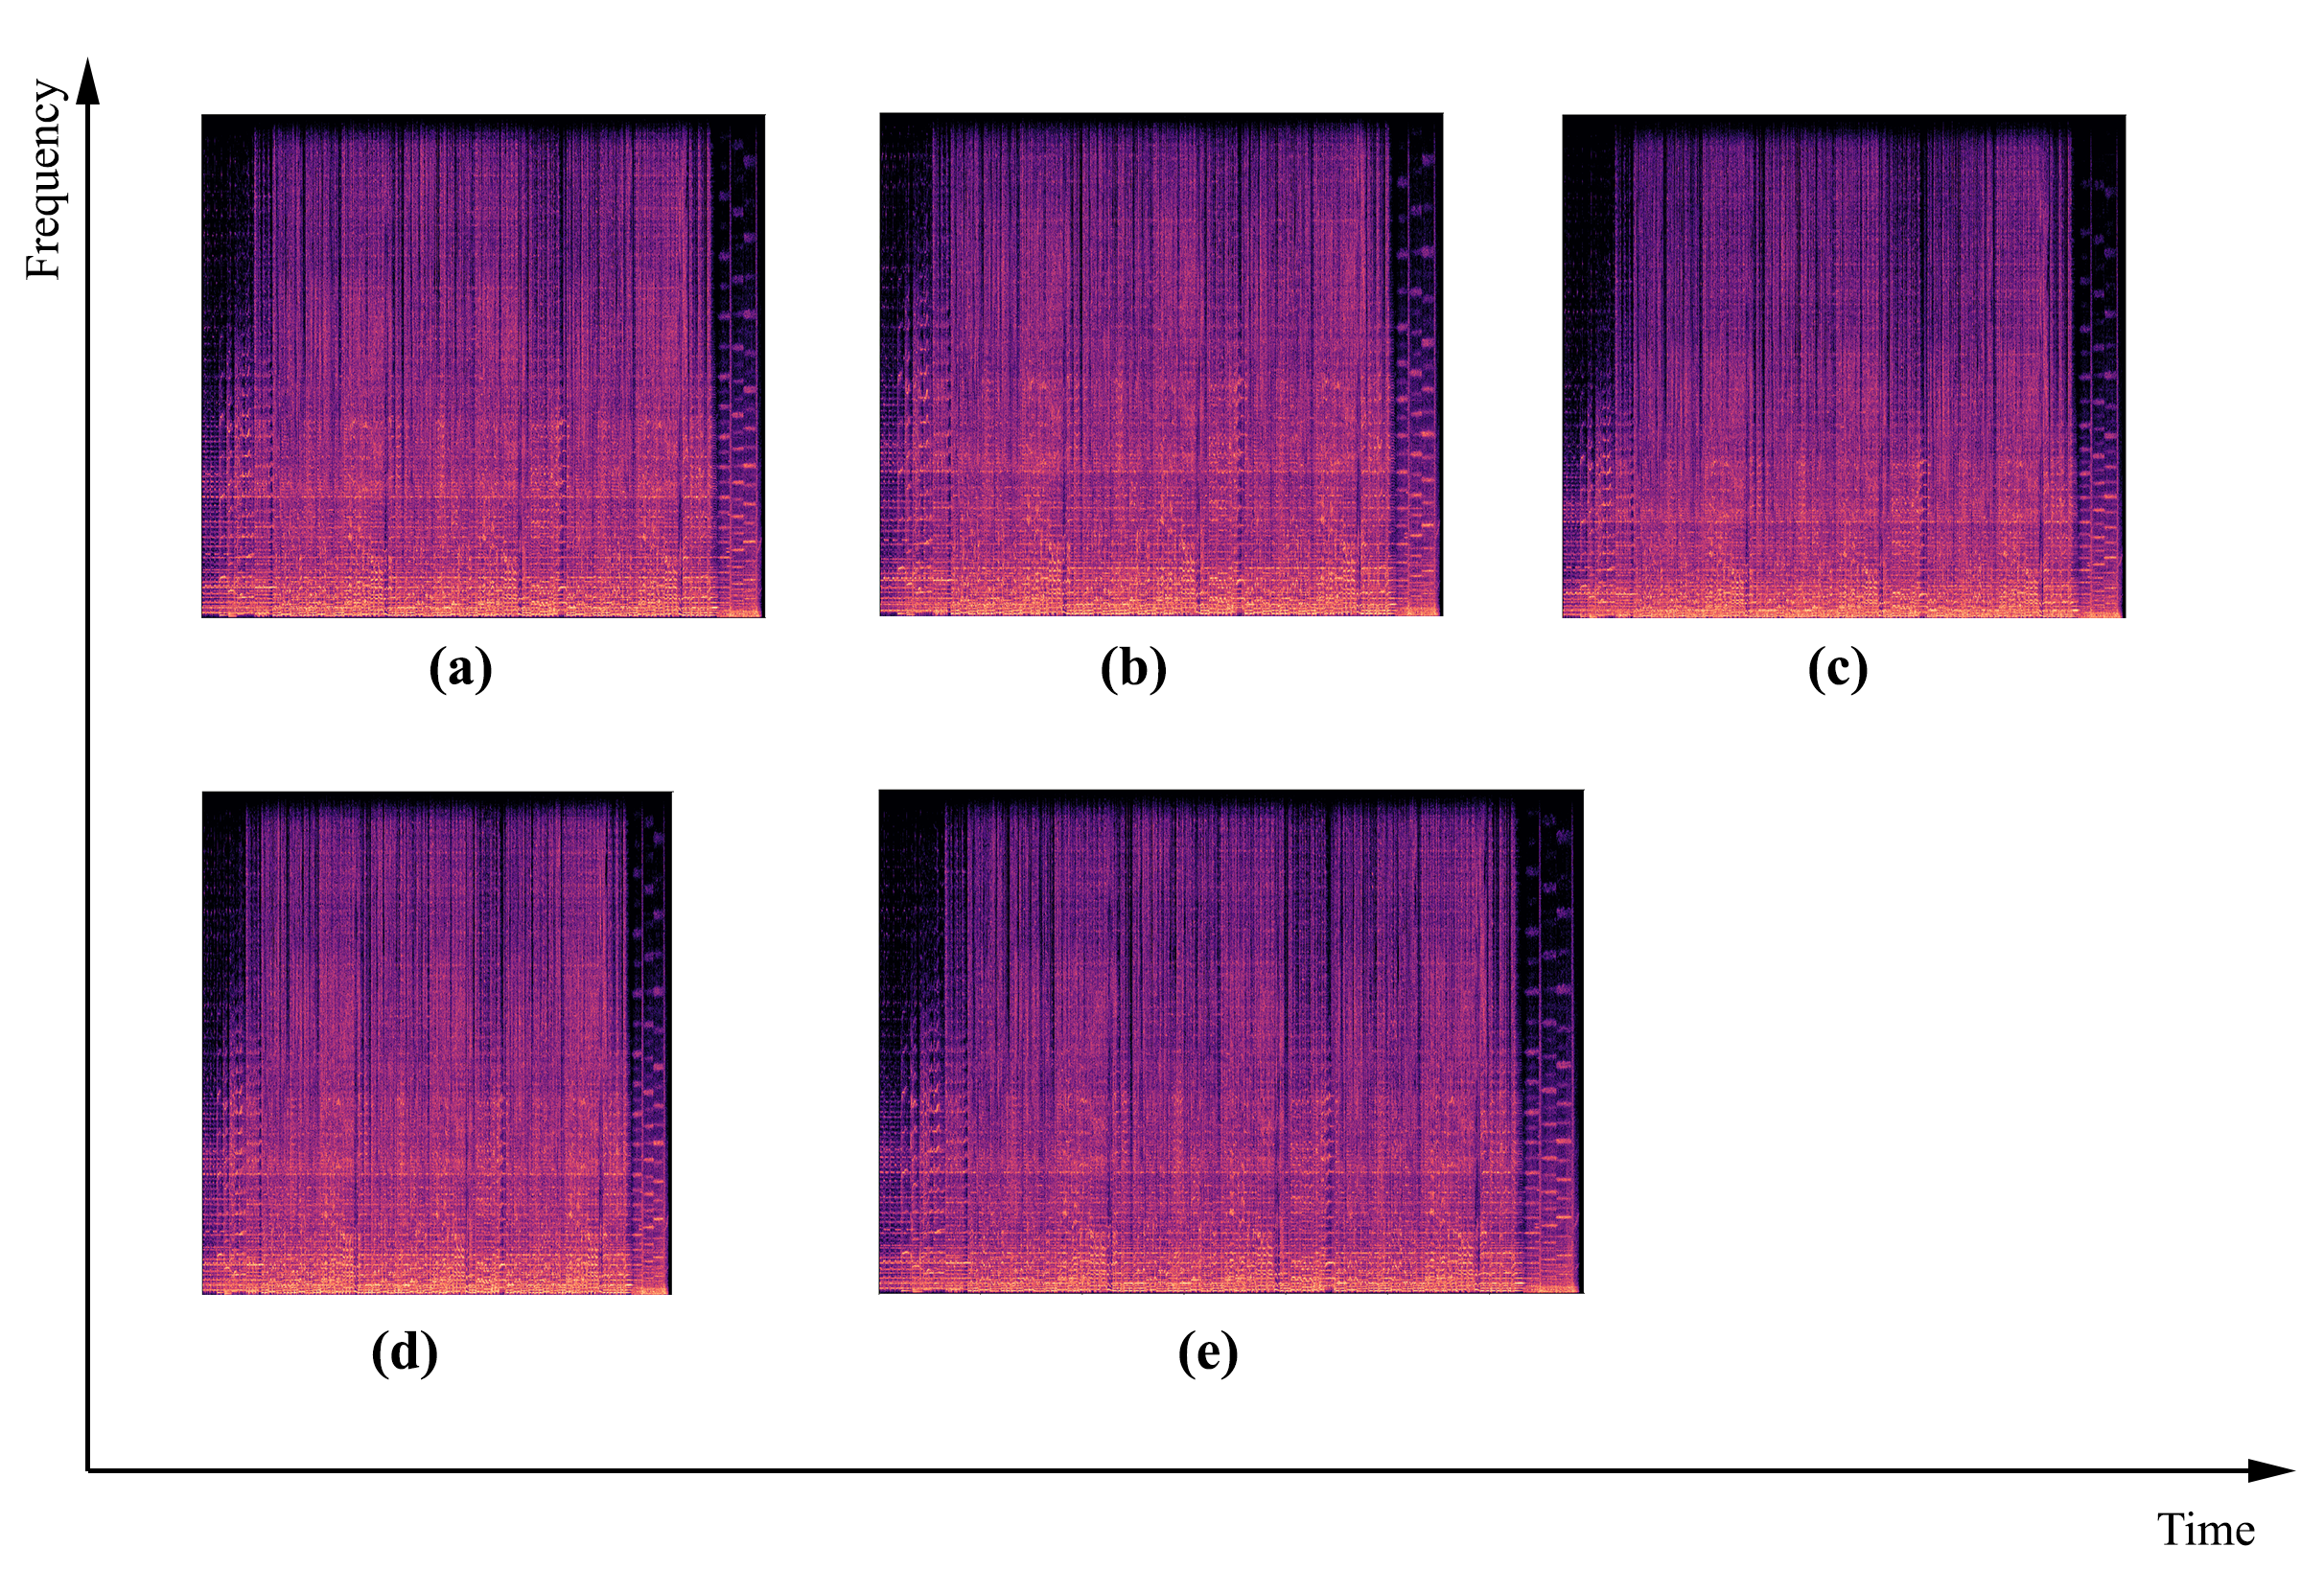
\includegraphics[scale=0.6]{spec_transform.png}
    \caption{Spectrogram transformations on audio enhancements. \textbf{(a)} is the spectrogram image of a original song. \textbf{(b)} 20\% 
    pitch increase, \textbf{(c)} 20\% pitch decrease, \textbf{(d)} 20\% tempo increase and \textbf{(e)} 20\% tempo decrease spectrogram images.}
    \label{fig:compare_spectrogram_design}
  \end{figure}

\subsection{Short Time Fourier Transform}

\ac{stft}\cite{Kehtarnavaz2008} is used to transform a signal from time domain to frequency domain as time domain signals
are unstable. When selecting key parameters 2048 bits long window was used with 50\% overlap as depicted in Figure 
\ref{fig:spectrogram_parameters}, in order to ensure that every part of a signal is represented in two windows.

\begin{figure}[H]
    \centering
    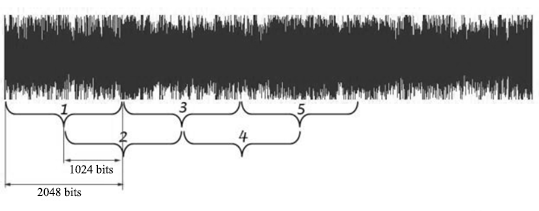
\includegraphics[scale=0.8]{parameters.png}
    \caption{Key parameters on \ac{stft}. 2048 bits long window with 1024 bits long overlapping area.}
    \label{fig:spectrogram_parameters}
  \end{figure}

  \ac{stft} is often visualized using its spectrogram\cite{Kehtarnavaz2008}, which is an intensity plot of \ac{stft} magnitude over time. 
  The generated spectrogram is converted to a color image as shown in Figure \ref{fig:spectrogram_design}. Axis labels and ticks are removed to stop
  identification of them as key points in feature extracting step. 

  \begin{figure}[H]
    \centering
    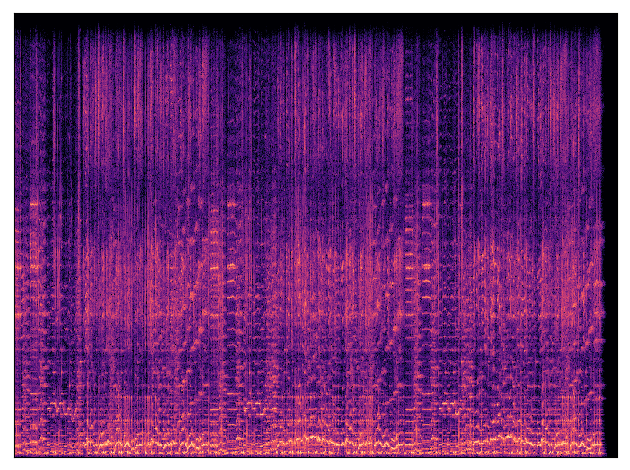
\includegraphics[scale=0.5]{spectrogram.png}
    \caption{Generated colour image of a spectrogram}
    \label{fig:spectrogram_design}
  \end{figure}

\subsection{SIFT Descriptor Extraction}

\ac{sift} is used in computer vision to identify scale invariant features of an image. \ac{sift} features are invariant to image rotation,
scale alterations and illumination\cite{Lowe2004}. The \ac{sift} feature extractor used in this method consists of four main steps.
\begin{enumerate}
  \item Scale space extrema detection: Gaussian filters of different scales are applied to the image and potential key points are selected
  as local minima or maxima of the \ac{dog} for multiple scales.
  \item Keypoint localization: Keypoints that have low contrast or those that are poorly located along edges
  are filtered out.
  \item Orientation assignment: One or more orientations are assigned to each keypoint based on local image gradient. 
  \item Keypoint descriptor generation: Orientation histograms are created for 4 x 4 pixel neighborhoods for each keypoint.
  Each histogram consists 8 bins, hence (4 x 4 x 8) 128 dimensional descriptor is generated.
\end{enumerate}

\ac{sift} generate (\(\text{No of Keypoints} \times 128\)) dimension matrix for each spectrogram. In average, more than 1000 keypoints 
are identified from a single spectrogram as shown in the Figure \ref{fig:spectrogram_keypoints}.  

  \begin{figure}[H]
    \centering
    \includegraphics[scale=0.5]{sift_keypoints.jpg}
    \caption{Identified keypoints in a SIFT spectrogram}
    \label{fig:spectrogram_keypoints}
  \end{figure}

\subsection{SIFT Descriptor Matching}

Music identification is facilitated by matching a feature matrix of a query audio clip with a feature matrix of a original song. Final goal
of the matching is to identify the count of keypoints that are matched with the original song. Identification of matching keypoints achieved
by taking 2 nearest keypoints to a query keypoint and checking whether the distance to the closest keypoint is lesser than 
the \(0.75 \times \text{distance to the 2nd closest keypoint}\). Those keypoints which were matched can be visualized as shown in the 
Figure \ref{fig:spectrogram_match}.

\begin{figure}[H]
    \centering
    \includegraphics[scale=0.3]{spec_match.png}
    \caption{Matched keypoints of two spectrograms}
    \label{fig:spectrogram_match}
  \end{figure}

\subsection{Thresholding}

Final step is to determine whether that query audio clip has the matched original song or not. It's archived by a thresholding method. 
In the begging keypoint count was used as the threshold measure. But it had drawbacks such as when query audio is variable length
number of keypoints identified will be different which eventually leads to different number of keypoints matched. Hence just using
keypoint count as a threshold measure didn't work as finding a generalized threshold value is really different. 

Therefore a ratio based threshold measure was recommended. Where we consider both number of keypoints that matched and initially identified 
keypoints count. Keypoint ratio can be obtained by below equation.

\begin{align*}
    \text{Keypoint ratio} &= \frac{\text{Matched keypoint count}}{\text{Keypoints generated for query audio clip}}\\
\end{align*}

Keypoint ratio can be used as better threshold measure as we can find generalized threshold value irrespective of length of the query audio clip. 
Threshold value selection and results will be discussed on Section \ref{section:results}. 